\documentclass[]{article}
\usepackage{lmodern}
\usepackage{amssymb,amsmath}
\usepackage{ifxetex,ifluatex}
\usepackage{fixltx2e} % provides \textsubscript
\ifnum 0\ifxetex 1\fi\ifluatex 1\fi=0 % if pdftex
  \usepackage[T1]{fontenc}
  \usepackage[utf8]{inputenc}
\else % if luatex or xelatex
  \ifxetex
    \usepackage{mathspec}
  \else
    \usepackage{fontspec}
  \fi
  \defaultfontfeatures{Ligatures=TeX,Scale=MatchLowercase}
\fi
% use upquote if available, for straight quotes in verbatim environments
\IfFileExists{upquote.sty}{\usepackage{upquote}}{}
% use microtype if available
\IfFileExists{microtype.sty}{%
\usepackage{microtype}
\UseMicrotypeSet[protrusion]{basicmath} % disable protrusion for tt fonts
}{}
\usepackage[unicode=true]{hyperref}
\hypersetup{
            pdfborder={0 0 0},
            breaklinks=true}
\urlstyle{same}  % don't use monospace font for urls
\usepackage{longtable,booktabs}
% Fix footnotes in tables (requires footnote package)
\IfFileExists{footnote.sty}{\usepackage{footnote}\makesavenoteenv{long table}}{}
\usepackage{graphicx,grffile}
\makeatletter
\def\maxwidth{\ifdim\Gin@nat@width>\linewidth\linewidth\else\Gin@nat@width\fi}
\def\maxheight{\ifdim\Gin@nat@height>\textheight\textheight\else\Gin@nat@height\fi}
\makeatother
% Scale images if necessary, so that they will not overflow the page
% margins by default, and it is still possible to overwrite the defaults
% using explicit options in \includegraphics[width, height, ...]{}
\setkeys{Gin}{width=\maxwidth,height=\maxheight,keepaspectratio}
\IfFileExists{parskip.sty}{%
\usepackage{parskip}
}{% else
\setlength{\parindent}{0pt}
\setlength{\parskip}{6pt plus 2pt minus 1pt}
}
\setlength{\emergencystretch}{3em}  % prevent overfull lines
\providecommand{\tightlist}{%
  \setlength{\itemsep}{0pt}\setlength{\parskip}{0pt}}
\setcounter{secnumdepth}{0}
% Redefines (sub)paragraphs to behave more like sections
\ifx\paragraph\undefined\else
\let\oldparagraph\paragraph
\renewcommand{\paragraph}[1]{\oldparagraph{#1}\mbox{}}
\fi
\ifx\subparagraph\undefined\else
\let\oldsubparagraph\subparagraph
\renewcommand{\subparagraph}[1]{\oldsubparagraph{#1}\mbox{}}
\fi

% set default figure placement to htbp
\makeatletter
\def\fps@figure{htbp}
\makeatother


\date{}

\begin{document}

\emph{Lombalgia }

La lombalgia è caratterizzata da un dolore penetrante che \emph{insorge
lentamente o improvvisamente con o senza irradiazione} alla natica o
lungo la gamba ed è associata a concomitante limitazione della mobilità.

A seconda della localizzazione si può avere:

\begin{itemize}
\item
  \begin{quote}
  \textbf{LOMBOSCIATALGIA} ovvero irradiazione dolorosa al di sotto del
  ginocchio. In questo caso la sintomatologia nervosa parte dalla
  regione glutea e raggiunge la tibiotarsica quindi coinvolge tutto
  l'arto inferiore (interessamento di L5 o S1)
  \end{quote}
\end{itemize}

\begin{itemize}
\item
  \begin{quote}
  \textbf{LOMBOCRURALGIA} ovvero irradiazione dolorosa all'inguine e
  alla faccia anteriore della coscia (interessamento di L2, L3, L4).
  \end{quote}
\end{itemize}

N.B. Quando parliamo di spazi parliamo di un interessamento della radice
nervosa che sta al di sotto. Ad esempio se parliamo di spazio tra L5 ed
S1, la compressione è della radice sacrale quindi di S1.

Per avere un'irradiazione dolorosa alla coscia potrebbero essere
interessati gli spazi L1-L2, L2-L3, L3-L4.

Avremo dei segnalatori che ci possono far pensare che ci sia un
interessamento a quei livelli e questi segnalatori sono i riflessi.

La lombalgia è un sintomo abbastanza comune a diverse patologie sia in
ambito reumatologico sia in ambito ortopedico come l'osteoartrosi della
colonna e la spondilite anchilosante.

L'incidenza della lombalgia dipende dal fatto che il segmento lombare
del rachide presenta \emph{caratteristiche anatomiche e funzionali} tali
da determinare una sua \emph{ipersollecitazione} e quindi
\emph{renderlo} più suscettibile alla sintomatologia algica. Tali
caratteristiche sono

\begin{itemize}
\item
  \begin{quote}
  Maggiore suscettibilità alle sollecitazioni statiche
  \end{quote}
\end{itemize}

\begin{itemize}
\item
  \begin{quote}
  Minore sviluppo del legamento longitudinale posteriore in larghezza
  quindi in spessore
  \end{quote}
\end{itemize}

\begin{itemize}
\item
  \begin{quote}
  Tratto a maggior mobilità del rachide
  \end{quote}
\end{itemize}

\begin{itemize}
\item
  \begin{quote}
  Oltre a sopportare il carico dell'intero rachide, le vertebre lombari
  sono sottoposte a sollecitazioni di scivolamento dovute
  all'inclinazione della base del sacro.
  \end{quote}
\end{itemize}

L'espressione più importante della lombalgia è legata alla
sintomatologia dolorosa: il dolore può essere più o meno variabile e più
o meno penetrante a seconda che ci sia o meno un interessamento della
radice nervosa.

Normalmente la lombalgia ha un'eziologia benigna, tende ad autolimitarsi
nel giro di 2-3 settimane a meno che non sia una forma particolarmente
acuta.

Epidemiologia

Secondo indagini epidemiologiche l'85\% della popolazione (indagine
ISTAT) ha avuto almeno una volta nella vita un episodio di lombalgia.

Normalmente nel 15\% dei casi la durata dei sintomi supera le 2
settimane mentre in una percentuale bassa (tra il 5 e il 10\%) tende a
cronicizzare e quindi si riduce l'intensità del dolore, ma diviene
costante.

È molto comune tra i lavoratori: il 50\% dei giorni di lavoro persi sono
legati a patologie muscolo-scheletriche come la lombalgia.

Colpisce uomini e donne in egual misura e più spesso tra i 30 e i 50
anni.

Causa un grado di invalidità variabile e soggettiva con aumento dei
costi individuali e sociali.

Da qui l'attenzione particolare al discorso della movimentazione dei
carichi durante l'attività lavorativa. Al primo posto per ricorrenza di
lombalgia c'è il personale infermieristico, per mobilitazione dei
pazienti e quindi attività ripetitive.

In Germania sono molto attenti sotto questo punto di vista e ci sono
catene di montaggio che presentano i pezzi in posizioni diverse per
permettere variazioni di movimento.

\emph{Nel 85\%-90\% dei casi la guarigione avviene nell'arco di tre mesi
circa; il 40\%-50\% di questi pazienti tendono alla Lombalgia
Recidivante. }

\emph{Il 10\%-15\% dei casi diverranno lombalgici cronici con vario
grado di invalidità.}

Classificazione

C'è una classificazione riconosciuta a livello internazionale che
suddivide la lombalgia in base al tempo in:

\begin{itemize}
\item
  \begin{quote}
  \emph{Forma acuta}: dolore che dura 2-4 settimane e tende ad
  autolimitarsi
  \end{quote}
\end{itemize}

\begin{itemize}
\item
  \begin{quote}
  \emph{Forma subacuta}: dolore che può durare da 4 settimane fino a 3
  mesi
  \end{quote}
\end{itemize}

\begin{itemize}
\item
  \begin{quote}
  \emph{Forma cronica}: dolore che supera i 3 mesi
  \end{quote}
\end{itemize}

\begin{itemize}
\item
  \begin{quote}
  \emph{Forma ricorrente}: dopo un periodo di remissione di almeno 6
  mesi. Alcuni però pensano che si possa parlare di forma ricorrente
  anche dopo un periodo di remissione di 2 mesi. Quando si hanno 3-4
  episodi nell'arco dell'anno c'è sicuramente una condizione di
  lombalgia ricorrente.
  \end{quote}
\end{itemize}

Quando la lombalgia diventa cronica il \emph{dolore è sicuramente meno
intenso} rispetto alla forma acuta, \emph{però è costante.}

\emph{La classificazione delle sindromi del dolore lombare prende invece
in considerazioni le possibili cause di insorgenza e vede:}

\begin{itemize}
\item
  \emph{Un 20\% di cause specifiche: vertebrali o viscerali}
\item
  \emph{80\% di cause non specifiche: }
\end{itemize}

\begin{itemize}
\item
  \emph{Vita sedentaria}
\item
  \emph{Forma fisica scadente}
\item
  \emph{Sovrappeso}
\item
  \emph{Stress}
\item
  \emph{Depressione, perdita di autostima}
\item
  \emph{Lavoro statico, ripetitivo e insoddisfacente}
\item
  \emph{Allenamenti fisici eccessivi nello sport }
\end{itemize}

Eziopatogenesi

Dal punto di vista eziopatogenetico ci sono forme meccaniche, forme non
meccaniche, forme di origine viscerale.

\begin{itemize}
\item
  \begin{quote}
  \textbf{LOMBALGIA MECCANICA}: rappresenta il 95-97\% delle forme di
  lombalgia. Ulteriormente suddivisa in base alle cause in:
  \end{quote}
\end{itemize}

\begin{itemize}
\item
  \emph{Lombalgia meccanica da cause specifiche} e sono il 12\% dei
  casi. Tra le cause ci sono: frattura osteoporotica, ernia discale,
  stenosi vertebrale, spondilolistesi, grave scoliosi, ipercifosi
\item
  \emph{Lombalgia meccanica da cause comuni} e sono 85\% dei casi.
  \emph{Le cause più comuni sono vita sedentaria, forma fisica scadente,
  sovrappeso, stress, depressone, lavoro statico, ripetitivo e
  insoddisfacente.} E' generalmente legata ad attività ripetitive: c'è
  una predisposizione costituzionale, ma è legata a processi artrosici
  vertebrali ovvero situazioni in cui si hanno instabilità vertebrali
  legate a spondilolisi e spondilolistesi vertebrale o ernie discali.
\end{itemize}

\begin{itemize}
\item
  \begin{quote}
  \textbf{LOMBALGIA NON MECCANICA}: rappresenta 1\% dei casi. Le cause
  più comuni sono: neoplasie, metastasi, ascessi epidurali, spondisciti,
  osteomielite, artrite reumatoide, Paget osseo, mieloma multiplo,
  spondilite anchilosante, polimialgia reumatica.
  \end{quote}
\end{itemize}

\begin{itemize}
\item
  \begin{quote}
  \textbf{LOMBALGIA DI ORIGINE VISCERALE}: rappresenta il 2\% dei casi.
  Le cause sono: patologie vascolari (aneurisma dell'aorta addominale),
  patologie del pancreas (neoplasie, pancreatite), patologie retro
  peritoneali (neoplasie, ematomi, fibrosi), patologie renali
  (neoplasie, ulcera, retto colite ulcerosa), patologie apparato
  genitale (neoplasie, endometriosi, prostatite, gravidanza
  extrauterina).
  \end{quote}
\end{itemize}

Valutazione clinica

La valutazione clinica del paziente si avvale di:

\begin{itemize}
\item
  \begin{quote}
  Anamnesi
  \end{quote}
\end{itemize}

\begin{itemize}
\item
  \begin{quote}
  Esame obiettivo generale, \emph{posturale e specifico della colonna
  vertebrale}
  \end{quote}
\end{itemize}

\begin{itemize}
\item
  \emph{Indagini strumentali: radiografia standard, TAC, RMN, EMG, MOC,
  scintigrafia ossea, esami ematochimici, altre indagini necessarie per
  escludere patologie correlate. }
\end{itemize}

\begin{itemize}
\item
  \begin{quote}
  Esame neurologico
  \end{quote}
\end{itemize}

Questi rappresentano il primo step per giungere ad una diagnosi di
patologia rachidea o di altre patologie (diagnosi differenziale).

La diagnosi può risultare difficile ed è importante formularne una
corretta infatti spesso le lombalgie vengono erroneamente classificate
come forme comuni e trattate in forma aspecifica, soprattutto
sintomatica. Altrettanto importante è identificare condizioni
potenzialmente gravi o che necessitano di intervento chirurgico.

In definitiva la diagnosi è importante per indirizzare il trattamento
farmacologico/strumentale/riabilitativo.

Anamnesi

Con l'anamnesi occorre:

\begin{itemize}
\item
  \begin{quote}
  Valutare i fattori di rischio:
  \end{quote}
\end{itemize}

\begin{itemize}
\item
  \emph{Lavoro sedentario}
\item
  \emph{Lavoro fisicamente impegnativo}
\item
  \emph{Frequenti sollevamenti}
\item
  \emph{Frequenti rotazioni e/o flessioni del tronco}
\item
  \emph{Scarsa cura del proprio corpo}
\item
  \emph{Stress posturali}
\item
  \emph{Obesità}
\item
  \emph{Fumo}
\item
  \emph{Comportamento poco attento alla salute}
\end{itemize}

\begin{itemize}
\item
  \begin{quote}
  Valutare come vengono descritti il tipo di dolore quindi gli
  \emph{aggettivi} che vengono utilizzati.
  \end{quote}
\end{itemize}

\begin{itemize}
\item
  \begin{quote}
  Individuare pazienti con segni non organici (ansioso, rassegnato o
  ipocondriaco).
  \end{quote}
\end{itemize}

\begin{itemize}
\item
  \begin{quote}
  Individuare situazioni psicosociali negative.
  \end{quote}
\end{itemize}

\begin{itemize}
\item
  \begin{quote}
  Precedenti episodi lombalgici.
  \end{quote}
\end{itemize}

\begin{itemize}
\item
  \begin{quote}
  Stato di salute generale.
  \end{quote}
\end{itemize}

\begin{itemize}
\item
  \begin{quote}
  Precedenti interventi chirurgici.
  \end{quote}
\end{itemize}

\begin{itemize}
\item
  \begin{quote}
  Individuare fattori favorenti o scatenanti come:
  \end{quote}
\end{itemize}

\begin{itemize}
\item
  Il tipo di attività lavorativa ed il tempo libero quindi momento e
  modo di inizio dei sintomi. Occorre approfondire gli stress specifici
  che tali attività comportano sul rachide come pesi, posture, durata,
  assenze per lombalgia
\item
  Recenti traumi, gravidanza, movimenti abnormi e sovraccarichi
  funzionali e altre patologie dell'apparato locomotore.
\end{itemize}

I microtraumi si scatenano nel tempo.

Particolare attenzione va riservata al dolore. Esiste una scala per la
valutazione del dolore detta \emph{\emph{Visual Analogic Scale}} che va
da 0 ovvero assenza dolore a 10 ovvero dolore intollerabile. E' molto
importante capire il tipo di dolore e come si manifesta perché
condiziona il tipo di trattamento. \emph{Bisogna valutare:}

\begin{itemize}
\item
  \emph{\emph{Dolore}} che aumenta con tosse, starnuto e sforzo. Questo
  indica una componente irritativa radicolare con aumento della
  pressione sulla radice nervosa. La lombalgia dà compressione del disco
  sulla dura madre. La lombosciatalgia dà compressione del disco sulla
  radice\emph{. }
\item
  \emph{\emph{Distribuzione del dolore}}: varia a seconda
  dell'interessamento della radice.
\item
  \emph{Modalitàà di insorgenza e durata (acuto/cronico), circostanze di
  peggioramento e di miglioramento. }
\end{itemize}

\begin{itemize}
\item
  \emph{Tipo, severità, intensità, orario e durata del dolore. }
\item
  \emph{Localizzazione precisa ed irradiazione del dolore}
\item
  \emph{Concomitanza con altri sintomi. }
\item
  \emph{Presenza di malattie connettivali, metaboliche, cardiovascolari,
  neurologiche e gastro-intestinali}
\item
  \emph{Presenza di disturbi depressivi, ansia, stress psicologico,
  problemi familiari, economico-sociali, lavorativi.}
\end{itemize}

Infine bisogna definire la tipologia del \textbf{\emph{dolore}}:

\begin{itemize}
\item
  \begin{quote}
  \textbf{DOLORE MECCANICO}. Le caratteristiche sono:
  \end{quote}
\end{itemize}

\begin{itemize}
\item
  Insorgenza o aumento con l'attività fisica
\item
  Riduzione con il riposo o assumendo posizioni antalgiche
\item
  Non è costante durante la giornata: peggio al mattino e alla sera
  mentre va meglio di notte.
\end{itemize}

In questo occorrerà un analgesico

\begin{itemize}
\item
  \begin{quote}
  \textbf{DOLORE NEUROPATICO-CHIMICO-INFIAMMATORIO}. È un dolore di tipo
  chimico-infiammatorio:
  \end{quote}
\end{itemize}

\begin{itemize}
\item
  Insorge anche a riposo
\item
  È costante e non circadiano
\item
  Non si giova di posizioni antalgiche
\item
  Non trova beneficio col riposo
\item
  Compare nella seconda metà della notte
\item
  Dapprima è attenuato dai movimenti, successivamente ricompare per
  l'affaticamento
\item
  Non è localizzato, ma irradiato.
\end{itemize}

\begin{quote}
In questo caso occorrerà usare un FANS anche se già da alcuni anni in
Europa si usano trattamenti combinati che prevedono molecole in cui c'è
un'associazione di analgesico e antinfiammatorio: si usa soprattutto
l'associazione paracetamolo-ibuprofene.
\end{quote}

\emph{Nel caso di \emph{dolore a insorgenza acuta} sarà necessario
valutare le eziologie, tra le quali si elencano alcune condizioni gravi,
che richiedono ulteriori indagini e spesso intervento immediato: }

\emph{- \textbf{Sindrome della cauda equina }}

\emph{È necessaria una decompressione chirurgica d'urgenza. La causa di
solito è una pressione estrinseca della cauda equina da parte di
un'ernia centrale massiva del nucleo polposo. Altre possibili cause
comprendono: ascesso ed ematoma epidurale, trauma, tumore epidurale. I
segni sono ritenzione urinaria, anestesia a sella (insensibilitàà di
ano, perineo, genitali), deficit bilaterali sensitivi o motori }

\emph{- \textbf{Frattura della colonna lombare }}

\emph{Dall'anamnesi emergono un trauma grave, come un incidente
stradale, o un trauma minore, come il sollevamento di carichi, all'esame
obiettivo si valutano il dolore e possibili sintomi e segni neurologici;
richiede immobilizzazione ed intervento di stabilizzazione vertebrale }

\emph{- \textbf{Tumore o infezione }}

\emph{Più frequenti nelle età \textgreater{}50 anni o \textless{} 20
anni, anamnesi di neoplasia, sintomi generali di febbre, brividi e calo
ponderale inspiegato; indagine di fattori di rischio infettivi quali
l'uso di corticosteroidi sistemici, trapianto, HIV; il dolore peggiora
in posizione supina, può essere grave di notte o non remittente. }

Nella valutazione clinica del paziente si possono valutare anche aspetti
più sofisticati come:

\begin{itemize}
\item
  \begin{quote}
  \emph{\emph{Disturbi del sonno}} (risveglio, farmaci ipnoinducenti).
  Ad esempio il risveglio con dolore che aumenta camminando coincide con
  una patologia grave nell'87\% dei casi
  \end{quote}
\end{itemize}

\begin{itemize}
\item
  \begin{quote}
  \emph{\emph{Febbre}} (processo infiammatorio)
  \end{quote}
\end{itemize}

\begin{itemize}
\item
  \begin{quote}
  \emph{\emph{Rapida perdita di peso}}
  \end{quote}
\end{itemize}

\begin{itemize}
\item
  \begin{quote}
  \emph{\emph{Precedente neoplasia}}
  \end{quote}
\end{itemize}

\begin{itemize}
\item
  \begin{quote}
  \emph{\emph{Forza muscolare}}: in caso di perdita di forza per esempio
  agli arti, ci può essere interessamento non solo della radice nervosa,
  ma anche del midollo e quindi si può avere una mielopatia (occorre in
  tal caso un intervento chirurgico di decompressione).
  \end{quote}
\end{itemize}

\begin{itemize}
\item
  \begin{quote}
  \emph{\emph{Sensibilità}}: Se c'è una riduzione del riflesso o
  un'areflessia, c'è una compressione importante idem se il riflesso è
  ipereccitato o se c'è un riflesso che si mantiene e che sembra sia
  ridondante.
  \end{quote}
\end{itemize}

\begin{itemize}
\item
  \begin{quote}
  \emph{\emph{Deambulazione}}
  \end{quote}
\end{itemize}

\begin{itemize}
\item
  \begin{quote}
  \emph{\emph{Sintomi legati}} ad incontinenza urinaria o alterazione
  della sensibilità perineale (radici sacrali -- sindrome cauda equina,
  ma solo quando c'è una \emph{\emph{compressione importante}}, come
  un'ernia espulsa).
  \end{quote}
\end{itemize}

\emph{Esempio riportato: ragazzo di 16 anni che da più di un anno soffre
di dolore inguinale a dx con diagnosi di pubalgia. }

\emph{In realtà tramite RMN dorsale e lombare è stata fatta poi una
diagnosi di compressione radicolare tra T7 e T10, L5-S1, L2-L3; ernia
discale T7-T8; protrusione discale L2-L3 e protrusione discale L5-S1.
Infatti in anamnesi risultava che egli era caduto con la moto quando era
piccolo, 7-8 anni fa}

Esame obiettivo della colonna lombare

\begin{enumerate}
\def\labelenumi{\arabic{enumi}.}
\item
  \emph{ISPEZIONE.} Può evidenziare la presenza di:
\end{enumerate}

\begin{itemize}
\item
  \emph{Deformità della colonna quali scoliosi, cifosi, lordosi,
  dismetrie}
\item
  \emph{Eventuale assunzione di atteggiamenti antalgici per esempio
  scoliosi antalgiche}
\item
  \emph{Osservazione della deambulazione e nello specifico:}
\end{itemize}

\begin{itemize}
\item
  Come il paziente si muove
\item
  Come si postura
\item
  Come si siede
\item
  Come si spoglia (movimenti, gestualità non naturali)
\item
  La valutazione complessiva della postura
\item
  La valutazione durante la marcia (cammino sui talloni e sulle punte)
\end{itemize}

\begin{quote}
Il \emph{\emph{cammino sui talloni e sulle punte}} serve a valutare che
non ci siano deficit importanti. Se il soggetto non riesce, significa
che c'è una componente irritativa radicolare.

Una delle manovre da fare per vedere se c'è una compressione della prima
radice sacrale (quindi dello spazio L5-S1) è valutare la forza
dell'estensore comune delle dita e dell'estensore proprio dell'alluce
dalla parte in cui il paziente sente l'irradiazione dolorosa. Se c'è un
deficit allora vuol dire che c'è un interessamento della radice L5-S1 e
ci sarà anche un'iporeflessia.
\end{quote}

Bisogna osservare il paziente in \emph{visione frontale, laterale e
posteriore} per vedere la simmetria e le eventuali asimmetrie che
possono essere legate al dolore come ad esempio le scoliosi antalgiche.

\begin{itemize}
\item
  \emph{Visione frontale:} le spalle e il bacino sono orizzontali e
  simmetrici; le clavicole uguali; i capezzoli alla stessa altezza;
  naso, ombelico e inguine in appiombo tra i malleoli tibiali.
\item
  \emph{Visione l\emph{aterale: per}} apprezzare le curvature sagittali:
  cifosi e lordosi; per valutare che la lordosi lombare sia adeguata e
  che non ci siano per esempio eventuali iperlordosi o ipercifosi a
  livello dorsale.
\item
  \emph{Visione posteriore:} per la simmetria di spalle, scapole e
  triangoli della taglia, appiombo tra occipite C7 e linea interglutea,
  deviazione scoliotica.
\end{itemize}

\begin{enumerate}
\def\labelenumi{\arabic{enumi}.}
\item
  \emph{MOBILITA'. Bisogna valutare:}
\end{enumerate}

\begin{itemize}
\item
  \emph{La mobilità articolare attiva e passiva della colonna e degli
  arti.} Nello specifico valutare i movimenti che il soggetto riesce a
  compiere in tutti i piani articolari, considerando ampiezza, armonia e
  qualità del movimento. Nel dettaglio:
\end{itemize}

\begin{itemize}
\item
  Flessione: si possono usare test specifici tipo quello di Schober per
  misurare la distanza tra le vertebre e vedere se la distanza aumenta
  durante la flessione o no. Ancora si può valutare la distanza dal
  suolo delle dita della mano in flessione: se il soggetto va a dx ha un
  accorciamento importante della colonna posteriore o una sintomatologia
  dolorosa che gli impedisce di flettere.
\item
  Estensione: si possono fare movimenti di estensione e fare pressioni
  sulle apofisi spinose per verificare che non ci sia dolore
  localizzato. Spesso ci sono forme di instabilità vertebrale da
  spondilolistesi che vengono identificate in questo modo e andando a
  palpare posteriormente si ha la sensazione che ci sia uno scalino: i
  processi spinosi non si riescono a palpare bene, ma si sente questo
  scalino che è l'avanzamento di quella vertebra.
\item
  Rotazione (in piedi o seduto)
\item
  Inclinazione laterale I movimenti vengono comparati con quelli contro
  laterali.
\end{itemize}

\begin{itemize}
\item
  \emph{Dolorabilità all'esecuzione di manovre specifiche}
\item
  \emph{Riduzione della mobilità articolare}
\end{itemize}

\begin{enumerate}
\def\labelenumi{\arabic{enumi}.}
\item
  \emph{PALPAZIONE}. Il paziente è in piedi o in posizione prona, meglio
  con un cuscino al di sotto dell'addome. E' un esame specifico che
  serve per individuare gli spazi discali che in genere si vedono bene a
  meno che non si tratti di soggetti obesi. \emph{Inoltre si valuta la
  sensibilità locale in tutte le aree del dolore riferito (inguine,
  ischio crurali, addome e gran trocantere)}
\end{enumerate}

Tramite la palpazione dei processi trasversi si può trovare il
\textbf{\emph{segno dello scalino}}. Infine si può fare la palpazione
dei punti di Valleix e la palpazione delle articolazioni sacro-iliache
per cercare dolore e/o dolorabilità.

\begin{enumerate}
\def\labelenumi{\arabic{enumi}.}
\item
  \emph{Valutazione del \emph{trofismo, tonicità e forza muscolare}}
\item
  \emph{Valutazione dell'\emph{equilibrio} e \emph{posturale globale}}
\end{enumerate}

Distribuzione della sintomatologia parestesica in base
all'interessamento della radice nervosa

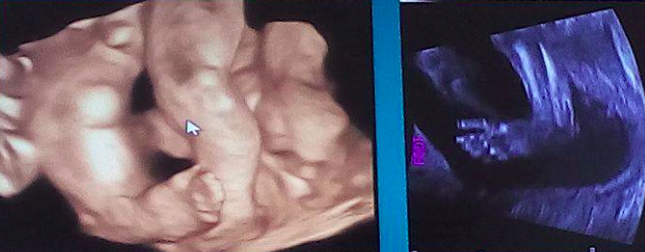
\includegraphics[width=4.30208in,height=3.77083in]{media/image1.png}

Come si può vedere dalle tavole che mostrano i dermatomeri:

\begin{itemize}
\item
  S1 va a prendere anche tutto il piede sulla parte esterna
\item
  L5 prende la parte centrale del piede con le prime tre dita
\item
  L4 la parte malleolare del piede
\end{itemize}

A volte sintomi localizzati a questi livelli, possono essere legati a
patologie discali.

Ci sono diversi soggetti con sintomatologia dolorosa al tallone
(tallodinie), in cui, con esame radiografico, si evidenzia un piccolo
aspetto di sperone calcaneale, ma perché sia uno sperone

\begin{quote}
Calcaneale deve essere uno sperone importante ed anteriore che possa
comprimere la fascia plantare. È molto probabile che quel soggetto possa
avere una protrusione: un'ernia discale tra L5 e S1. Cosi come molte
metatarsalgie possono essere legate a questo aspetto.
\end{quote}

Le metatarsalgie legate a possibili neuromi di Morton possono essere
legate a patologia radicolare di S1. Di neuromi di Morton non se ne
vedono molti, spesso l'esame non li mette in evidenza.

Test neurologici

Ci sono manovre e test neurologici che provocano reazione dolorosa del
paziente per uno stiramento delle radici nervose e che quindi mettono in
evidenza l'interessamento della radice. Tra queste c'è la
\textbf{\emph{manovra di Lasegue}}: il paziente è supino, flessione
dell'anca a 90° ed estensione della gamba sulla coscia (nervo sciatico).

C'è anche la \textbf{\emph{manovra di Wassermann Boschi}} per il nervo
crurale: paziente prono ed anca estesa e si fa una graduale flessione
della gamba sulla coscia (nervo crurale).

Nel dettaglio:

\begin{itemize}
\item
  Se c'è un interessamento della quarta radice lombare quindi dello
  spazio L3-L4, si ha un'iporeflessia rotulea che a volte può essere
  bilaterale quindi il soggetto può avere avuto in passato la stessa
  sintomatologia con un dolore localizzato prima da una parte e poi
  dall'altra poiché spesso l'ernia o la protrusione è mediana o
  paramediana. \emph{Mediana} significa che può estrinsecarsi a destra e
  a sinistra; \emph{paramediana} può estrinsecarsi lateralizzandosi a
  destra o a sinistra
\item
  Se abbiamo interessamento della quinta radice lombare quindi L4-L5, i
  riflessi ci sono tutti. Il paziente ha una sintomatologia dolorosa che
  parte dal gluteo, scende lungo la coscia, si muove posteriormente,
  gira davanti e scende avanti fino a prendere le prime tre dita del
  dorso del piede. La localizzazione deve far pensare ad un difetto
  della sensibilità.
\item
  In caso di interessamento del livello L5-S1, avremo un'iporeflessia
  del riflesso achilleo e del riflesso medio plantare. Si fa la manovra
  per vedere la forza dell'estensore comune delle dita e dell'estensore
  proprio dell'alluce: il paziente si mette in decubito prono con la
  caviglia rivolta in alto e si fa resistenza. Anche il paziente stesso
  facendolo attivamente potrebbe non riuscire a prendere la caviglia e
  c'è una flessione maggiore dal lato opposto.
\end{itemize}

\begin{quote}
\emph{\textbf{\emph{Valutazione delle radici nervose nella sciatica
(presenza di lombo sciatalgia nel paziente)}}}
\end{quote}

\begin{longtable}[]{@{}llll@{}}
\toprule
\begin{quote}
\emph{\textbf{Radice nervosa}}
\end{quote} & \begin{quote}
\emph{\textbf{Dermatomero}}
\end{quote} & \begin{quote}
\emph{\textbf{Esame motorio}}
\end{quote} & \begin{quote}
\emph{\textbf{Commento}}
\end{quote}\tabularnewline
\midrule
\endhead
\begin{quote}
\emph{L4}
\end{quote}

\emph{(Liv. Discale L3-L4)} & \begin{quote}
\emph{Faccia mediale del polpaccio fino alla parte mediale del piede,
prime 2 dita}
\end{quote} & \begin{quote}
\emph{Tibiale anteriore, posteriore, quadricipite femorale, medio
gluteo, tensore della fascia lata}
\end{quote} & \begin{quote}
\emph{La funzionalità della radice nervosa viene valutata esaminando la
forza del tibiale ant. che controlla la dorsiflessione e l'inversione
del piede}
\end{quote}\tabularnewline
\begin{quote}
\emph{L5}

\emph{(l.d. L4-L5)}
\end{quote} & \begin{quote}
\emph{Dorso del piede (parte laterale arto inf.)}
\end{quote} & \begin{quote}
\emph{Tibiale anteriore, estensore lungo}

\emph{Dell'alluce, grande gluteo, ischiocrurali, estensore lungo delle
dita}
\end{quote} & \begin{quote}
\emph{Esaminare la forza dell'estensore lungo dell'alluce facendo
resistenza all'estensione sull'articolazione metetarsofalangea;
valutazione della forza dei muscoli grande gluteo, estensori lungo e
breve delle dita con deambulazione sui talloni}
\end{quote}\tabularnewline
\begin{quote}
\emph{S1 (l.d. L5-S1)}
\end{quote} & \begin{quote}
\emph{Pianta, tallone e margine laterale del piede}
\end{quote} & \begin{quote}
\emph{Gastrocnemio, grande gluteo, ischio crurali, muscoli del piede,
peroneo lungo, peroneo breve}
\end{quote} & \begin{quote}
\emph{Valutazione della forza muscolare del gastrosoleo e dei flessori
plantari, valutazione mediante deambulazione sulle punte}
\end{quote}\tabularnewline
\begin{quote}
\emph{S2}
\end{quote} & \begin{quote}
\emph{Posteriore mediale della gamba inferiore e superiore}
\end{quote} & \begin{quote}
\emph{Flessore lungo delle dita, dell'alluce, muscoli del piede}
\end{quote} & \begin{quote}
\emph{Qualsiasi deformità dell'avampiede o delle dita indica la
possibilità che vi sia un problema su S2}
\end{quote}\tabularnewline
\begin{quote}
\emph{S3}
\end{quote} & \begin{quote}
\emph{Porzione mediale delle natiche}
\end{quote} & \begin{quote}
\emph{Aiuta ad alimentare la muscolatura intrinseca del piede}
\end{quote} &\tabularnewline
\bottomrule
\end{longtable}

Diagnosi differenziale

Quando c'è una lombocruralgia, bisogna fare una \emph{diagnosi
differenziale con la patologia dell'anca} perché una coxartrosi
importante dà una sintomatologia sovrapponibile a quella di una
lombocruralgia quindi va valutata:

\begin{itemize}
\item
  La flessione dell'anca
\item
  La rotazione dell'anca comparandola con quella contro laterale
\item
  Occorre fare una radiografia del bacino.
\end{itemize}

Nella patologia dell'anca si ha:

\begin{itemize}
\item
  Dolore inguinale o nell'area quadricipite,
\item
  Valutazione passiva ROM anca
\item
  Minore ROM in intrarotazione ed abduzione
\item
  Minor flessione e limitazione dell'estensione
\item
  Dolore alle rotazioni passive.
\end{itemize}

Un'altra \emph{diagnosi differenziale} va fatta \emph{con le patologie
dell'articolazione sacroiliaca}: spondilite anchilosante, traumi,
patologie da sovraccarico. La patologia sacro-iliaca comprende:

\begin{itemize}
\item
  Dolore dopo il parto, traumi
\item
  Dolore in zona sacro-iliaca, intermittente e a volte proiettato
  all'inguine o alla parete posteriore della coscia
\item
  Dolore al cammino, a volte dolore notturno o al cambio di posizione.
\end{itemize}

Un'altra patologia possibile è la \textbf{compressione del muscolo
piriforme} che si verifica in soggetti che fanno ciclismo, atletica,
saltatori in alto:

\begin{itemize}
\item
  E' un dolore correlato ad uno sforzo (corsa, cammino)
\item
  Spesso irradiato al ginocchio e non lombare senza altri segni
  neurologici
\item
  Aumenta durante la corsa e il cammino
\item
  È un dolore palpatorio (esplorazione rettale)
\item
  Sì esacerba all'extrarotazione dell'anca contro resistenza e
  all'intrarotazione passiva dell'anca.
\end{itemize}

\begin{quote}
Normalmente il dolore scompare con un'infiltrazione locale di
anestetico. Si fa il \emph{\textbf{\emph{test alla lidocaina}}} per la
diagnosi differenziale. Se il test è positivo non è un'irradiazione
legata ad una radice nervosa, ma ad uno sforzo e ad un interessamento
del muscolo piriforme.
\end{quote}

Diagnosi strumentale

La diagnosi strumentale si fa per iperlordosi, aumento dell'angolo
lombosacrale, rettilineizzazione, scoliosi, difetti di transizione
lombo-sacrale, fratture, lussazioni, spondilolistesi, spondilolisi,
artrosi (osteofiti, sindesmofiti, malattia di Baarstrup), osteoporosi
(\textless{}40\% massa, assottigliamento della corticale, deformazione a
lente biconcava e/o striature verticali dei corpi vertebrali, crolli),
riduzione dello spazio intervertrebale, tumori.

\begin{itemize}
\item
  \begin{quote}
  \textbf{Rx}: non necessaria entro le prime 4-6 settimane dall'inizio
  della sintomatologia lombalgica semplice. Proiezioni:
  \end{quote}
\end{itemize}

\begin{itemize}
\item
  \emph{Antero-posteriore}
\item
  \emph{Latero-laterale}
\item
  \emph{In posizione supina}
\item
  \emph{Oblique} per forami, articolazioni posteriori, spondilolisi
\item
  Dinamiche in flesso-estensione per sublussazione ed instabilità.
\end{itemize}

\begin{quote}
Secondo le linee guida della Società Internazionale di Medicina
Riabilitativa, la radiografia nel paziente con lombalgia al primo
episodio non andrebbe fatta. Eccetto che in condizioni particolari: il
paziente anziano con comorbilità importanti, se c'è stata caduta
precedente, se ci sono componenti di familiarità per altre patologie. In
tutti gli altri casi si fa un trattamento e se a distanza di 2-3
settimane dopo il trattamento farmacologico non c'è risposta magari si
fa un approfondimento diagnostico. Anche se in realtà tutti fanno fare
una radiografia per tutelarsi. Percorso definito dall'azienda
ospedaliera per i pazienti che arrivano in pronto soccorso per patologie
del rachide: vengono trattati in PS in acuto poi vengono inviati alla
medicina riabilitativa. Prima si attua un trattamento farmacologico e
poi riabilitativo.
\end{quote}

\begin{itemize}
\item
  \begin{quote}
  \textbf{TC}. applicabile al segmento L3-S1, tagli sagittali,
  trasversali e per i forami. Migliore visualizzazione delle strutture
  ossee e dei loro rapporti col canale neurale. Si può ricorrere alla
  TAC nel caso di fratture, artrosi, ernie, stenosi del canale,
  neoplasie.
  \end{quote}
\end{itemize}

\begin{itemize}
\item
  \begin{quote}
  \textbf{RMN}: migliore visualizzazione dei tessuti molli e dei
  rapporti tra disco e nervo. È più sensibile.
  \end{quote}
\end{itemize}

\begin{itemize}
\item
  \begin{quote}
  \textbf{Scintigrafia ossea}: può essere utilizzata in casi molto
  specifici. Per rachialgie diffuse, prevalentemente notturne, mal
  localizzabili, nel sospetto di neoplasie, spondilodisciti, fratture
  occulte, artrosi severa.
  \end{quote}
\end{itemize}

\begin{itemize}
\item
  \begin{quote}
  \textbf{Elettromiografia:} trova ottima indicazione dove si sospetta
  un interessamento radicolare (radicolopatie). Si può ricorrere ad un
  esame ad ago per analizzare la conduzione nervosa sensitiva e motoria
  e l'attività muscolare (a riposo, a sforzo massimo, a sforzo minimo).
  Si richiede nei casi con durata dopo le 6-8 settimane.
  \end{quote}
\end{itemize}

Trattamento

\emph{\textbf{GLI OBIETTIVI DELLA RIABILITAZIONE NELLA LOMBARDIA}}

\emph{- Trattare il dolore con mezzi che riducano il riposo al letto e
la dipendenza dai farmaci. }

\emph{- Migliorare la funzionalità vertebrale e rieducare la postura. }

\emph{- Insegnare una corretta ergonomia vertebrale nella vita
quotidiana e nel lavoro. }

\emph{- Insegnare al paziente l'autogestione delle manifestazioni a
carattere cronico ed infondere fiducia nelle proprie capacità fisiche. }

\emph{- Ritorno veloce alle normali attività lavorative e domestiche. }

\textbf{\emph{Trattamento della lombalgia comune acuta/subacuta}} (circa
7 giorni). Prima di tutto occorre rassicurare il paziente sulla causa,
sui fattori di rischio quindi consigliare di rimanere attivi eseguendo
attività fisica controllata. Al contrario di quanto detto in passato
quando il riposo era consigliato assolutamente però il movimento aiuta
nelle forme e nei modi in cui è possibile farlo. \emph{In generale il
riposo a letto è consigliato per non più di 2 giorni. Si può ricorrere a
un lombostato per un breve periodo e comunque solo di giorno}. In caso
di dolore e limitazione funzionale importante consigliare una terapia
farmacologica: \emph{analgesici, FANS e miorilassanti. Infine si può
ricorrere anche a mesoterapia antalgica, infiltrazioni antalgiche
paravertebrali corticosteroidee e blocco delle faccette articolari.}

\begin{quote}
\textbf{Trattamento della Lombalgia Acuta con fisioterapia }
\end{quote}

\begin{itemize}
\item
  \emph{Mezzi fisici antalgici: ipertermia, tecarterapia, laser, TENS,
  correnti diadinamiche, ultrasuoni, magnetoterapia.}
\item
  \emph{Massoterapia decontratturante. La \textbf{terapia manipolativa}
  e le \textbf{trazioni vertebrali} possono essere effettuate in
  particolari casi molto selezionati con indicazione specifica e
  precisa. Le trazioni vertebrali è meglio non usarle se c'è uno
  sfiancamento del disco e quindi un'ernia.}
\end{itemize}

\begin{quote}
\emph{Possono essere indicate la manipolazione e la trazione vertebrale
quando c'è una patologia del disco al fine di diminuire la compressione
locale. Devono essere eseguite da personale altamente specializzato,
meglio se da personale medico. Il SSN riconosce la terapia riabilitativa
sotto la dizione di mano medica per evitare problemi di tipo medico
legale, non essendoci un albo per i chiropratici osteopati. }
\end{quote}

\begin{itemize}
\item
  \emph{Insegnare posture corrette antalgiche e di scarico vertebrale. }
\item
  \emph{Manipolazioni/mobilizzazioni. }
\item
  \emph{Esercizi antalgici. }
\item
  \emph{Training autogeno.}
\item
  \emph{Uso di ortesi. Le \textbf{ortesi e i corsetti lombosacrali} si
  usano quando dobbiamo scaricare la colonna vertebrale e dare un
  supporto per diminuire il carico. }
\end{itemize}

\textbf{\emph{Mezzi fisiocinesiterapici antalgici: }}

1. \emph{Ipertermia}

\emph{2. Laserterapia (sembra abbia poco effetto) }

\emph{3. T.E.N.S.}

\emph{4. Dyadinamic}

\emph{5. Ultrasuoni}

\emph{6. Magnetoterapia}

\emph{7. Elettrostimolazioni muscolari}

\emph{8. Massoterapia decontratturante }

\emph{9. Trazioni/manipolazioni vertebrali }

\textbf{\emph{Trattamento della lombalgia cronica}.} Rivalutare il
paziente, consigliare esercizio fisico e approccio
cognitivo-comportamentale con un programma multidisciplinare.

\begin{itemize}
\item
  Test di Waddel (fattori psicosociali)
\item
  Scale di disabilità Roland Morris
\item
  Disability Questionnaire.
\item
  Owestry Disability Index.
\end{itemize}

\begin{quote}
Nella forma cronica è importante consigliare attività fisica con
esercizi di rinforzo muscolare ed educare il paziente ad eseguire
esercizi a domicilio per mantenere un buon tono muscolare. C'è tipo la
Back School, la ``scuola della schiena'', che dà indicazioni su come
muovere la schiena, come comportarsi nel movimentare i carichi e
sollevare i pesi. Il trattamento è così riassunto:
\end{quote}

\begin{itemize}
\item
  \begin{quote}
  \emph{TERAPIA FARMACOLOGICA} (analgesici, FANS)
  \end{quote}
\end{itemize}

\begin{itemize}
\item
  \emph{TERAPIA FISICA} (TENS, US, LASER).
\end{itemize}

\begin{itemize}
\item
  \emph{MASSOTERAPIA. }
\end{itemize}

\begin{itemize}
\item
  \emph{MANIPOLAZIONI, MESOTERAPIA, AGOPUNTURA. ORTESI}
\end{itemize}

\begin{itemize}
\item
  \begin{quote}
  \emph{RIEDUCAZIONE POSTURALE GLOBALE}
  \end{quote}
\end{itemize}

\begin{itemize}
\item
  \emph{BACK SCHOOL/ IDROKINESITERAPIA. }
\item
  \emph{INFILTRAZIONE PERIDURALE. }
\end{itemize}

\begin{itemize}
\item
  \emph{TRATTAMENTO CHIRURGICO. }
\end{itemize}

La \textbf{Back School} è un programma di prevenzione e trattamento
finalizzato ad un gruppo di persone con lezioni teorico-pratiche.

Un'altra tecnica è la \textbf{Core-Stability} oppure il \textbf{Pilates}
(a metà strada tra Back School e la riabilitazione posturale).

Una volta fatto il trattamento farmacologico, posso fare terapia fisica
strumentale: la \textbf{TENS} è l'unica terapia strumentale consigliata
per la lombalgia con qualche minima evidenza di efficacia. L'ultrasuono,
invece, non ha mostrato evidenze scientifiche in termini di successo
terapeutico.

Il \textbf{Laser} potrebbe essere utile, ma a patto che chi fa la
diagnosi sia bravo a stabilire in quale fase usarlo: in fase acuta non
si utilizza poiché si va a riscaldare un tessuto infiammato.

La \textbf{Massoterapia} può dare benefici se c'è una contrattura e se
non c'è una componente radicolare.

Le \textbf{Manipolazioni} vanno bene se effettuate da personale
qualificato; l'osteopata va di moda, ma può andar bene se viene inserito
in un progetto riabilitativo identificato da uno specialista. Lo stesso
vale per il chiropratico.

La \textbf{Mesoterapia} è una buona tecnica che utilizza un cocktail di
farmaci iniettati localmente sottocute. Sì hanno gli stessi effetti se
somministriamo per via mesoterapia gli stessi farmaci che utilizziamo
per via orale, il vantaggio è che li somministriamo localmente e
somministriamo il 50\% in meno della dose.

Gli esercizi in acqua sono molto importanti come prevenzione secondaria.

\textbf{L' infiltrazione peridurale} solo nei casi estremi.

Gli \textbf{interventi chirurgici} su ernie discali lombari non si
effettuano quasi mai a meno che ci sia un trauma importante in cui
bisogna decomprimere immediatamente, i risultati sono migliorati, nel
70\% hanno buoni benefici.

La \textbf{kinesiterapia} è molto utile. Ha vantaggi dal punto di vista
preventivo e valore terapeutico per evitare la recidiva; ha come
obiettivi il miglioramento dell'articolarità, il potenziamento muscolare
selettivo e il corretto atteggiamento posturale; può potenziare i
muscoli per stabilizzare la colonna. Non usare in fase acuta e in
pazienti troppo anziani.

L'\textbf{idrokinesiterapia} permette il recupero da escursione
articolare ed un inizio precoce dell'attività di resistenza. Utilizzata
per analgesia, decontrazione, rilassamento, aumento dell'articolarità,
miglioramento della circolazione ed effetti psicologici.

Tecniche di riabilitazione posturale come la \textbf{Mc Kenzie}
propongono movimenti in iperestensione per aprire le vertebre e
aumentare gli spazi, ma attenzione: in alcune situazioni
l'iperestensione non va assolutamente fatta; è usata per rachialgie di
origine meccaniche; l'obiettivo è trattare l'episodio in corso e
prevenire recidive.

\emph{\emph{Rieducazione posturale globale}} la tecnica
\textbf{Mezieres-Suchard}: è una tecnica di stiramento globale che
coinvolge non solo il segmento affetto, ma anche i distretti muscolari
sopra e sottostanti. Si basa sul fatto che bisogna allungare le catene
muscolari accorciate, coordinare i movimenti con la respirazione
diaframmatica ed effettuare gli esercizi in espirazione dal momento che
c'è un collegamento tra le catene posturali quindi il rachide cervicale
è collegato al rachide lombare. I pazienti che hanno ernie lombari nel
90-95\% hanno la stessa localizzazione a livello cervicale.

Le infiltrazioni peridurali con corticosteroidi tipo 80 mg di
metilprednisolone (medrol) hanno risultati buoni. Nella genesi clinica
del dolore radicolare si possono poi riconoscere due componenti,
variamente sovrapposte, infiammatoria e neuropatica.

La \emph{componente infiammatoria} trae beneficio dall'azione del
cortisone che raggiunge con la peridurale il massimo di concentrazione
locale.

La \emph{componente neuropatica} che stimola il SNC e SNP con meccanismo
di feedback sul simpatico, causando vasocostrizione localizzata, viene
invece trattata dall'anestetico locale che blocca il simpatico.

L'\textbf{ossigeno-ozonoterapia} usa due tecniche: una
\emph{infradiscale} per aumentare lo spazio utilizzando l'effetto
pressorio dell'ossigeno-ozono (tra l'altro l'ozono ha un effetto
antiinfiammatorio importante) o \emph{infiltrazione sui forami di
comunicazione all'emergenza delle radici.}

\end{document}
